\chapter{Student Learning Objectives}\label{chap:slos}
This chapter consists of two major sections.  Section~\ref{sect:technicalSkills}
focuses on the technical skills you have learned during my time here at
Western.  Section~\ref{sect:socialSkills} focuses on the skills I have
acquired that are non-technical. The social skills section mainly focuses on my ethics course and my technical skills section focuses mainly on CS350.

\section{Technical Skills}\label{sect:technicalSkills}
By ``technical skills'' I mean not just programming languages, but paradigms, algorithms, and engineering methodologies that differentiate a good programmer from a hobbyist. Included in this section are three SLOs: Software Engineering, Algorithms, and Systems. Though at this time I've completed only Systems. The other sections will be filled as I progress through my major.

%\subsection{Software Engineering}\label{chap:softwareEngineering}
What is software engineering?  How does software engineering related to the
student learning objectives of being able to ``use the steps of the software
development process to create high-quality software''.  Summarize the key
topics.

Give an overview of this section.  What work samples will you include?
(You must include at least two.)  You can cite any references like
this~\cite{parks:samsfsoal:2009}.

\subsubsection{Name of Work Sample 1}
Give an introduction for the work sample and explain its context.  The
introduction for the work sample must be at least 50 words.

The work samples must address the student learning objectives addressed in
this section.  A work sample may be used to address more than one student
learning objective.  If you use the same work sample to address multiple
objectives, put it in the Appendix and reference it here.
There are a range of possible work that might be
included as work samples including parts of the software develop process
for a particular program (e.g., requirements specification, design documents,
test suites, and the program code itself), papers written, and
experimental or theoretical studies.  The work samples need not only
be from the current course.  You should remember to save your work when
you finish a course so that you can use that work as a work sample in
your portfolio later.

Depending on the length of the work sample, you may include it in-line in
this section, or include it in the appendix.  Listing~\ref{lst:sampleWorkSample4}
is an example of how to include a work sample in-line. (And that's how you
link to it.)

\begin{singlespace}
\begin{lstlisting}[float,
                   escapeinside='',
                   basicstyle=\ttfamily\footnotesize,
                   emphstyle=\textbf,
                   numberstyle=\tiny,
                   xleftmargin=.3cm,
                   language=java,
                   numbers=left,
                   numbersep=5pt,
                   firstnumber=auto,
                   stepnumber=1,
                   numberblanklines=true,
                   showspaces=false,
                   showstringspaces=false,
                   showtabs=false,
                   captionpos=b,
                   caption=Sample Java Source File,
                   label=lst:sampleWorkSample4]
public class Hello {
    public static void main(String[] args) {
        System.out.println("Hello, World!");
    }
}
\end{lstlisting}
\end{singlespace}

Here, some of your work samples might be diagrams.  For example,
Figure~\ref{fig:doctorUseCase3} is a use case diagram for a patient tracking
system. (And that's how you link to it.)

\begin{figure}
    \centering
    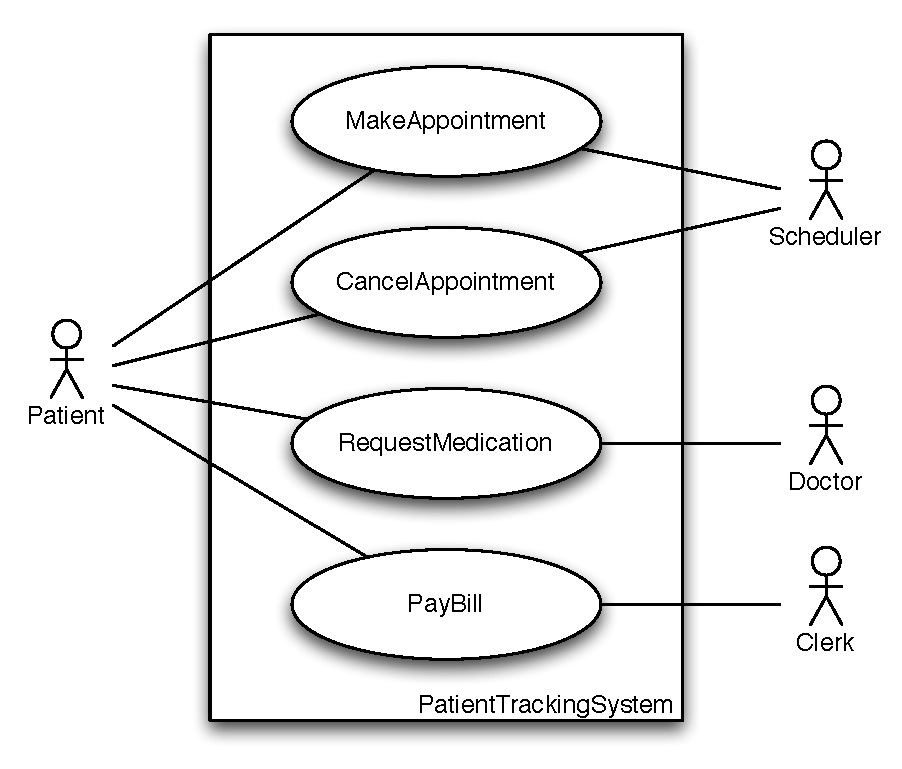
\includegraphics[width=4in]{figures/DoctorsOfficeUseCase}
    \caption{PatientTrackingSystem Use Case}
    \label{fig:doctorUseCase3}
\end{figure}

\subsubsection{Name of Work Sample 2}
Give an introduction for the work sample and explain its context.  The
introduction for the work sample must be at least 50 words.

Appendix~\ref{chap:appendixA} includes a long work sample.  (And that's how you
link to it.)

\subsubsection{Reflection}
In this section, you are to explain in your own words:
\begin{enumerate}
\item Your view of the meaning of the student learning objective
\item What aspect of each work sample addresses this student learning
      objective
\item An honest and accurate appraisal of your strengths and weaknesses at
      this point in your career with respect to this SLO.  It is unlikely
      that you have no weaknesses and it is also unlikely that you have no
      strengths with respect to this SLO.
\end{enumerate}

The length of this subsection must be at least 500 words.

%\subsection{Algorithms}
Why is it important for a computer scientist to be able ``to create and analyze
non-trivial algorithms''?  Summarize the key topics related to this SLO.

Give an overview of this section.  What work samples will you include?
(You must include at least two.)  You can cite any references like
this~\cite{parks:samsfsoal:2009}.

\subsubsection{Name of Work Sample 1}
Give an introduction for the work sample and explain its context.  The
introduction for the work sample must be at least 50 words.

The work samples must address the student learning objectives addressed in
this section.  A work sample may be used to address more than one student
learning objective.  If you use the same work sample to address multiple
objectives, put it in the Appendix and reference it here.
There are a range of possible work that might be
included as work samples including parts of the software develop process
for a particular program (e.g., requirements specification, design documents,
test suites, and the program code itself), papers written, and
experimental or theoretical studies.  The work samples need not only
be from the current course.  You should remember to save your work when
you finish a course so that you can use that work as a work sample in
your portfolio later.

Depending on the length of the work sample, you may include it in-line in
this section, or include it in the appendix.  Listing~\ref{lst:sampleWorkSample1}
is an example of how to include a work sample in-line. (And that's how you
link to it).

\begin{singlespace}
\begin{lstlisting}[float,
                   escapeinside='',
                   basicstyle=\ttfamily\footnotesize,
                   emphstyle=\textbf,
                   numberstyle=\tiny,
                   xleftmargin=.3cm,
                   language=java,
                   numbers=left,
                   numbersep=5pt,
                   firstnumber=auto,
                   stepnumber=1,
                   numberblanklines=true,
                   showspaces=false,
                   showstringspaces=false,
                   showtabs=false,
                   captionpos=b,
                   caption=Yet Another Sample Java Source File,
                   label=lst:sampleWorkSample1]
public class Hello {
    public static void main(String[] args) {
        System.out.println("Hello, World!");
    }
}
\end{lstlisting}
\end{singlespace}

\subsubsection{Name of Work Sample 2}
Give an introduction for the work sample and explain its context.  The
introduction for the work sample must be at least 50 words.

Appendix~\ref{chap:appendixA} includes a long work sample.  (And that's how you
link to it.)

Maybe you want to include a table of some experimental results?
Table~\ref{table:experimentalResults} shows an example of how to do that.
(And that's how you link to it.)

\begin{table}
\centering
\begin{tabular}{ll}
\textit{Label1} & \textit{Label2}\\
\hline \hline
Name            & value\\
Name            & value\\
Name            & value\\
Name            & value\\
\end{tabular}
\caption{Experimental Results}
\label{table:experimentalResults}
\end{table}

\subsubsection{Reflection}
In this section, you are to explain in your own words:
\begin{enumerate}
\item Your view of the meaning of the student learning objective
\item What aspect of each work sample addresses this student learning
      objective
\item An honest and accurate appraisal of your strengths and weaknesses at
      this point in your career with respect to this SLO.  It is unlikely
      that you have no weaknesses and it is also unlikely that you have no
      strengths with respect to this SLO.
\end{enumerate}

The length of this subsection must be at least 500 words.

\subsection{Systems}
It is vital for a computer scientist to understand how computer systems operate at the lowest level because it allows them not only to create better code but to create better systems. When one understands what their code is ultimately doing they can fine-tune it to perform much faster and more efficiently. In this section I have two work samples of MIPS assembly code and one example of C code demonstrating threading.

\subsubsection{AtoI}
This program shows my basic understanding of and ability to manipulate assembly code. It shows how to use system calls and how to go about allocating data for a program.While simple I feel it's necessary to include this because of it's relative importance to my overall portfolio. Demonstrating mastery of a language, while not necessarily inline with this SLOs goals is nevertheless very important.
You can see this program in Appendix~\ref{chap:appendixA}.

\subsubsection{Three Procedures}
For this assignment we were required to write three procedures, and a driver, in MIPS. The procedures were \texttt{strlen}, \texttt{strncpy}, and \texttt{mem\_align}. This program shows my understanding of low-level procedure calls: what needs to be passed, how, and what needs to be returned and how. Perhaps more importantly it shows what all needs to be kept track of when maintaining the executing environment across procedure calls, the stack pointer, the return address pointer, and so on.

Listing~\ref{stackstuff} shows how to go about manipulating the stack to store the registers according to the rules one follows when one invokes a procedure.
\lstset{language=[mips]Assembler,basicstyle=\footnotesize,numbers=left,numberstyle=\footnotesize,label=stackstuff}
\begin{lstlisting}
addi $sp, $sp, -16          # $sp-=4; /* allocate 4 words */
sw $s0, 0($sp)              # *($sp + 0) = $s0 /* save $s0 */
sw $s1, 4($sp)              # *($sp + 4) = $s1 /* save $s1 */
sw $s2, 8($sp)              # *($sp + 8) = $s2 /* save $s2 */
sw $s3, 12($sp)             # *($sp + 12) = $s3 /* save $s3 */
--------------------------------------------------------------
lw $s0, 0($sp)              # $s3 = *($sp + 0); /* restore $s0 */
lw $s1, 4($sp)              # $s3 = *($sp + 4); /* restore $s1 */
lw $s2, 8($sp)              # $s3 = *($sp + 8); /* restore $s2 */
lw $s3, 12($sp)             # $s3 = *($sp + 12); /* restore $s3 */
addi $sp, $sp, 16           # $sp+=4; /* deallocate 4 words */
\end{lstlisting}

You can see this entire program in Appendix~\ref{chap:appendixB}.

\subsection{BoundedBuffer}
This program was written for an assignment in CS370, Operating Systems. This program is most succinctly described as a thread-safe bounded circular buffer. Making use of the \textit{POSIX Threading} library this program provides a block of memory to which threads can write and read. If a thread attempts to write to the buffer, and the space available in the buffer is sufficient to hold the data the thread is writing, the thread will copy the data to the buffer and continue executing. However if the buffer is full on a write, or empty on a read, then the thread will block waiting for a read() or write() call to be made. Listing~\ref{bbh} shows the prototype of the bounded buffer as provided by Dr. Dalton.
\lstset{language=c,basicstyle=\footnotesize,numbers=left,numberstyle=\footnotesize,label=bbh}
\begin{lstlisting}
#ifndef BOUNDEDBUFFER_H
#define BOUNDEDBUFFER_H
#include <pthread.h>
typedef struct {
  char* data;
  int capacity;
  int start;
  int end;
  int size;
  pthread_mutex_t mutex;
  pthread_cond_t cond;
} BoundedBuffer;
void bufferInit(BoundedBuffer* buffer, int capacity);
void bufferWrite(BoundedBuffer* buffer, char* data, int count);
void bufferRead(BoundedBuffer* buffer, char* data, int count);
void bufferDeallocate(BoundedBuffer* buffer);
#endif
\end{lstlisting}

You can see the implementation of these methods in Appendix~\ref{chap:appendixC}.
\subsubsection{Reflection}
I believe that an understanding of systems is very important for a computer scientist to quote the textbook for CS350, \textit{Computer Organization And Design}, ``The performance of software systems is dramatically affected by how well software designers understand the basic hardware technologies at work in a system'' ~\cite{pat94}. In addition to that it is necessary for a computer scientist to understand the relationships between the software and hardware, the design choices, and the reasons for those design choices. 

Reflecting on my work from this area of computer science I can safely say I have a strong grasp of systems concepts. I understand pipelining, multi-cycle data paths, caches, virtual memory, assembly language, computer arithmetic, memory hierarchies, and I/O from the low level side. I do however wish I had a more complete understanding of caches. While I understand how they work and what they do, I don't understand the specifics of how a cache is set up.

On a higher level Andrew S. Tanenbaum's book \textit{Operating Systems: Design and Implementation}, the textbook for CS370, provides an excellent description of what someone dealing with higher level OS code should be proficient in: ``system calls, processes, IPC, scheduling, I/O, deadlocks, memory management, threads, filesystems, and more'' ~\cite{TanenbaumWoodhull08}. I believe I am proficient in all of these, and more. I had the benefit of learning C at a much higher level than I had ever dealt with before, shown in my third work sample from this SLO, which taught me quite a bit about programming. In addition dealing with MINIX in CS370 also taught me quite a bit about the low level code in an operating system. I am still lacking in some areas at the higher level though. I don't feel I have a firm understanding of DMA and I still don't entirely understand batch processing algorithms.

Despite the several pitfalls mentioned above I believe that my understanding of this topic is comprehensive.


\section{Social Skills}\label{sect:socialSkills}
By ``social skills'' I mean the ability to communicate effectively both in a technical setting and a non technical setting. This section includes three SLOs: Communication, Teamwork, and Ethics. Though at this time I've only completed Ethics. The other sections will be filled as I progress through my major.

%\subsection{Communication}
Why are communication skills important to computer scientists?  Why is it
important to be able to effectively express ideas in oral and written form?
Tell us why these things are important.  Summarize the key topics.

Give an overview of this section.  What work samples will you include?
(You must include at least two.)  You can cite any references like
this~\cite{parks:samsfsoal:2009}.

\subsubsection{Name of Work Sample 1}
Give an introduction for the work sample and explain its context.  The
introduction for the work sample must be at least 50 words.

The work samples must address the student learning objectives addressed in
this section.  A work sample may be used to address more than one student
learning objective.  If you use the same work sample to address multiple
objectives, put it in the Appendix and reference it here.
There are a range of possible work that might be
included as work samples including parts of the software develop process
for a particular program (e.g., requirements specification, design documents,
test suites, and the program code itself), papers written, and
experimental or theoretical studies.  The work samples need not only
be from the current course.  You should remember to save your work when
you finish a course so that you can use that work as a work sample in
your portfolio later.

Depending on the length of the work sample, you may include it in-line in
this section, or include it in the appendix.  Listing~\ref{lst:sampleWorkSample2}
is an example of how to include a work sample in-line. (And that's how you
link to it.)

\begin{singlespace}
\begin{lstlisting}[float,
                   escapeinside='',
                   basicstyle=\ttfamily\footnotesize,
                   emphstyle=\textbf,
                   numberstyle=\tiny,
                   xleftmargin=.3cm,
                   language=java,
                   numbers=left,
                   numbersep=5pt,
                   firstnumber=auto,
                   stepnumber=1,
                   numberblanklines=true,
                   showspaces=false,
                   showstringspaces=false,
                   showtabs=false,
                   captionpos=b,
                   caption=Sample Java Source File,
                   label=lst:sampleWorkSample2]
public class Hello {
    public static void main(String[] args) {
        System.out.println("Hello, World!");
    }
}
\end{lstlisting}
\end{singlespace}

\subsubsection{Name of Work Sample 2}
Give an introduction for the work sample and explain its context.  The
introduction for the work sample must be at least 50 words.

Appendix~\ref{chap:appendixA} includes a long work sample.  (And that's how you
link to it.)

\subsubsection{Reflection}
In this section, you are to explain in your own words:
\begin{enumerate}
\item Your view of the meaning of the student learning objective
\item What aspect of each work sample addresses this student learning
      objective
\item An honest and accurate appraisal of your strengths and weaknesses at
      this point in your career with respect to this SLO.  It is unlikely
      that you have no weaknesses and it is also unlikely that you have no
      strengths with respect to this SLO.
\end{enumerate}

The length of this subsection must be at least 500 words.

%\subsection{Teamwork}
Why is it important for a computer scientist to be able to work well with
others?  Summarize the key topics.

Give an overview of this chapter.  What work samples will you include?
(You must include at least two.)  You can cite any references like
this~\cite{parks:samsfsoal:2009}.

\subsubsection{Name of Work Sample 1}
Give an introduction for the work sample and explain its context.  The
introduction for the work sample must be at least 50 words.

The work samples must address the student learning objectives addressed in
this section.  A work sample may be used to address more than one student
learning objective.  If you use the same work sample to address multiple
objectives, put it in the Appendix and reference it here.
There are a range of possible work that might be
included as work samples including parts of the software develop process
for a particular program (e.g., requirements specification, design documents,
test suites, and the program code itself), papers written, and
experimental or theoretical studies.  The work samples need not only
be from the current course.  You should remember to save your work when
you finish a course so that you can use that work as a work sample in
your portfolio later.

Depending on the length of the work sample, you may include it in-line in
this section, or include it in the appendix.  Listing~\ref{lst:sampleWorkSample6}
is an example of how to include a work sample in-line. (And that's how you
link to it.)

\begin{singlespace}
\begin{lstlisting}[float,
                   escapeinside='',
                   basicstyle=\ttfamily\footnotesize,
                   emphstyle=\textbf,
                   numberstyle=\tiny,
                   xleftmargin=.3cm,
                   language=java,
                   numbers=left,
                   numbersep=5pt,
                   firstnumber=auto,
                   stepnumber=1,
                   numberblanklines=true,
                   showspaces=false,
                   showstringspaces=false,
                   showtabs=false,
                   captionpos=b,
                   caption=Sample Java Source File,
                   label=lst:sampleWorkSample6]
public class Hello {
    public static void main(String[] args) {
        System.out.println("Hello, World!");
    }
}
\end{lstlisting}
\end{singlespace}


\subsubsection{Name of Work Sample 2}
Give an introduction for the work sample and explain its context.  The
introduction for the work sample must be at least 50 words.

Appendix~\ref{chap:appendixA} includes a long work sample.  (And that's how you
link to it.)

\subsubsection{Reflection}
In this section, you are to explain in your own words:
\begin{enumerate}
\item Your view of the meaning of the student learning objective
\item What aspect of each work sample addresses this student learning
      objective
\item An honest and accurate appraisal of your strengths and weaknesses at
      this point in your career with respect to this SLO.  It is unlikely
      that you have no weaknesses and it is also unlikely that you have no
      strengths with respect to this SLO.
\end{enumerate}

The length of this subsection must be at least 500 words.

%\subsection{Ethics}
Why is it important for a computer scientist to have a strong foundation in
ethics and ethical behavior?  Summarize the key topics.

Give an overview of this section.  What work samples will you include?
(You must include at least two.)  You can cite any references like
this~\cite{parks:samsfsoal:2009}.

\subsubsection{Name of Work Sample 1}
Give an introduction for the work sample and explain its context.  The
introduction for the work sample must be at least 50 words.

The work samples must address the student learning objectives addressed in
this section.  A work sample may be used to address more than one student
learning objective.  If you use the same work sample to address multiple
objectives, put it in the Appendix and reference it here.
There are a range of possible work that might be
included as work samples including parts of the software develop process
for a particular program (e.g., requirements specification, design documents,
test suites, and the program code itself), papers written, and
experimental or theoretical studies.  The work samples need not only
be from the current course.  You should remember to save your work when
you finish a course so that you can use that work as a work sample in
your portfolio later.

Depending on the length of the work sample, you may include it in-line in
this section, or include it in the appendix.  Listing~\ref{lst:sampleWorkSample3}
is an example of how to include a work sample in-line. (And that's how you
link to it.)

\begin{singlespace}
\begin{lstlisting}[float,
                   escapeinside='',
                   basicstyle=\ttfamily\footnotesize,
                   emphstyle=\textbf,
                   numberstyle=\tiny,
                   xleftmargin=.3cm,
                   language=java,
                   numbers=left,
                   numbersep=5pt,
                   firstnumber=auto,
                   stepnumber=1,
                   numberblanklines=true,
                   showspaces=false,
                   showstringspaces=false,
                   showtabs=false,
                   captionpos=b,
                   caption=Sample Java Source File,
                   label=lst:sampleWorkSample3]
public class Hello {
    public static void main(String[] args) {
        System.out.println("Hello, World!");
    }
}
\end{lstlisting}
\end{singlespace}


\subsubsection{Name of Work Sample 2}
Give an introduction for the work sample and explain its context.  The
introduction for the work sample must be at least 50 words.

Appendix~\ref{chap:appendixA} includes a long work sample.  (And that's how you
link to it.)

\subsubsection{Reflection}
In this section, you are to explain in your own words:
\begin{enumerate}
\item Your view of the meaning of the student learning objective
\item What aspect of each work sample addresses this student learning
      objective
\item An honest and accurate appraisal of your strengths and weaknesses at
      this point in your career with respect to this SLO.  It is unlikely
      that you have no weaknesses and it is also unlikely that you have no
      strengths with respect to this SLO.
\end{enumerate}

The length of this subsection must be at least 500 words.

